%===============================================================================
\section{Theory of Special Cosserat rods}


%===============================================================================
\subsection{Kinematics of Cosserat rods}

%-------------------------------------------------------------------------------
\begin{frame}
  \frametitle{Introduction to \st{special} Cosserat rods (part 1)}
  
  \vspace{-1em}
  \begin{figure}
    \centering
    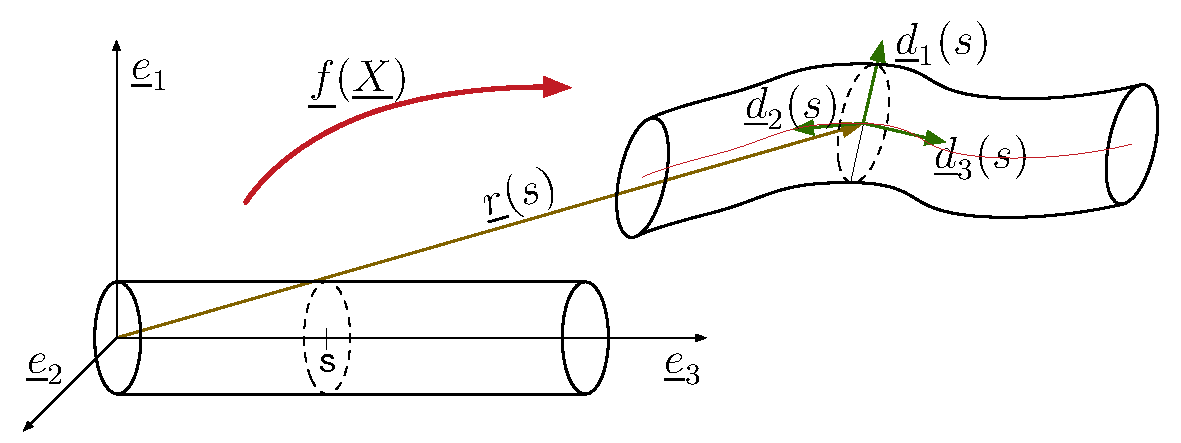
\includegraphics[width=20cm, keepaspectratio=true]{sections/cosserat_rods/images/Kinematics}
  \end{figure}
  
  remember: $s$ is the unique identifier for a particular cross section of the beam
  \vspace{0.6em}
  
  \textbf{kinematic quantities}:
  \begin{itemize}
    \item position of the deformed cross section $\underline{r}(s)$
    \item shearing of the deformed cross section $\underline{d}_1(s)$, $\underline{d}_2(s)$
    \item orientation of the deformed cross section $\underline{d}_3(s)$ \newline
      \null \quad (perpendicular to $\underline{d}_1(s)$ and $\underline{d}_2(s)$ $\rightarrow$ not independent)
    %\item $\doubleunderline{R}(s)$
  \end{itemize}
\end{frame}


%-------------------------------------------------------------------------------
\begin{frame}
  \frametitle{Introduction to \st{special} Cosserat rods (part 2)}

  \textbf{constrained deformation map}
  \begin{displaymath}
    \underline{f}(\underline{X}) = \underline{f}(X_1,X_2,X_3=s) = \underline{r}(s) + X_{\alpha} \, \underline{d}_{\alpha} \quad \text{with } \alpha \in \{1,2\}
  \end{displaymath}
  \vspace{1em}
  
  \textbf{consequences of the imposed kinematic constraints}
  \begin{itemize}
    \item cross sections remain flat
    \item straight lines within the cross section remain straight lines
    \item boundary of the cross section: circles are mapped to ellipses \newline
      \null \quad (not to arbitrary  curves in 2D)
    \item $\underline{d}_1(s)$ and $\underline{d}_2(s)$ are not perpendicular in the general case (shearing)
  \end{itemize}
\end{frame}


%===============================================================================
\subsection{Kinematics of Special Cosserat rods}


%-------------------------------------------------------------------------------
\begin{frame}
  \frametitle{What makes the Special Cosserat rod special?}

  \begin{itemize}
    \item $\underline{d}_1(s)$ and $\underline{d}_2(s)$ \textit{are} perpendicular and unit-normed
    \item hence $\left( \underline{d}_1, \underline{d}_2, \underline{d}_3 \right)$ form an orthonormal triad
  \end{itemize}
  \vspace{1em}
  
  \textbf{consequences}
  \begin{displaymath}
    \exists \: \doubleunderline{R}(s) \in SO(3) \: \forall s : \biggl( R: \left( \underline{e}_1, \underline{e}_2, \underline{e}_3 \right) \mapsto \left( \underline{d}_1, \underline{d}_2, \underline{d}_3 \right) \biggr)
  \end{displaymath}
  \begin{itemize}
    \item $\left( \underline{e}_1, \underline{e}_2, \underline{e}_3 \right)$ is called the global basis
    \item $\left( \underline{d}_1, \underline{d}_2, \underline{d}_3 \right)(s)$ is called the local basis or director basis at $s$
    \item $\underline{d}_i(s) = \doubleunderline{R}(s) \cdot \underline{e}_i$ \quad 
      ($\doubleunderline{R}$ : rotation matrix ; $SO(3)$ : special orthogonal matrix group)
  \end{itemize}
  \vspace{1em}
  
  \textbf{constrained deformation map}
  \begin{displaymath}
    \underline{f}(\underline{X}) = \underline{f}(X_1,X_2,X_3=s) = \underline{r}(s) + \doubleunderline{R}(s) \cdot (X_{\alpha} \, \underline{e}_{\alpha}) \quad \text{with } \alpha \in \{1,2\}
  \end{displaymath}
  
  \vspace{0.5em}
  $\rightarrow$ but the rigidity of the cross section is stiffening the beam!
\end{frame}


%-------------------------------------------------------------------------------
\begin{frame}
  \frametitle{Warp-mode on ;-)}
  
  we want to introduce warping of the cross section, \newline
  while at the same time keeping the director basis $\underline{d}_i$
  \vspace{0.6em}
  
  \textbf{modified deformation map}
  \begin{displaymath}
    \underline{f}(\underline{X}) = \underline{f}(X_1,X_2,X_3=s) = \underline{r}(s) + \doubleunderline{R}(s) \cdot (X_{\alpha} \, \underline{e}_{\alpha} + \underline{u}) \quad \text{with } \alpha \in \{1,2\}
  \end{displaymath}
  
  \vspace{0.3em}
  \textbf{geometric meaning of $\underline{u}$}
  \begin{itemize}
    \item $u_1$, $u_2$ : in-plane shrinking % TODO shrinking vs relative displacement
    \item $u_3$ : out-of-plane warping $\rightarrow$ cross section not planar anymore
    \item then $\underline{d}_1$, $\underline{d}_1$ represent the average orientation of the warped cross section
  \end{itemize}
  \vspace{0.6em}
  
  \textbf{what are our kinematic unknowns?}
  \begin{itemize}
    \item if $\underline{u} = \underline{u}(X_1,X_2,s)$ then we would be dealing with a 3D elasticity problem
    \item here we have $\underline{u}(X_1,X_2,\text{local strains})$, not a function of $s$ \newline (we will come back to this ...)
    \item $\underline{r}(s)$ and $\doubleunderline{R}(s)$ are the only kinematic unknowns!
  \end{itemize}
\end{frame}


%-------------------------------------------------------------------------------
\begin{frame}
  \frametitle{Rotations in 3D revisited}
  
  a \textbf{rotation about \textit{one} axis} is determined by
  \begin{itemize}
    \item axis of rotation given by $\underline{a}$ with $\norm{\underline{a}} = 1$
    \item angle of rotation $\Theta$
  \end{itemize}
  \vspace{0.6em}
  
  \textbf{composition of rotations}
  \begin{displaymath}
    \left( \underline{a}_1, \Theta_1 \right) + \left( \underline{a}_2, \Theta_2 \right) + \left( \underline{a}_3, \Theta_3 \right) + \dots = \left( \underline{a}_{eff}, \Theta_{eff} \right)
  \end{displaymath}
  note: ``$+$'' here denotes the composition of two rotations
  
  \begin{displaymath}
    \doubleunderline{R}_{eff} = \dots \cdot \doubleunderline{R}_3 \cdot \doubleunderline{R}_2 \cdot \doubleunderline{R}_1
  \end{displaymath}
  
  In the general case ($\underline{a}_i \neq \underline{a}_j \text{ for } i \neq j$) rotations do not commute!
  \vspace{1em}
  
  \textbf{example} (rotation about $\underline{e}_3$):
  \begin{displaymath}
    \Biggl( \underline{a} =
    \begin{bmatrix}
      0 \\ 0 \\ 1
    \end{bmatrix}, \Theta \Biggr) \quad \rightarrow \quad
    \doubleunderline{R} =
    \begin{bmatrix}
      +\cos(\Theta) & -\sin(\Theta) & 0 \\
      +\sin(\Theta) & +\cos(\Theta) & 0 \\
      0 & 0 & 1
    \end{bmatrix}
  \end{displaymath}
\end{frame}

%-------------------------------------------------------------------------------
\begin{frame}
  \frametitle{Axis-angle representation of rotations in 3D}
  
  from the axis-angle representation
  \begin{displaymath}
    \Biggl( \underline{a} =
    \begin{bmatrix}
      a_1 \\ a_2 \\ a_3
    \end{bmatrix}, \Theta \Biggr)
  \end{displaymath}
  we obtain the corresponding rotation matrix
  \begin{displaymath}
    \doubleunderline{R} = \exp(\Theta \cdot \doubleunderline{a})  
  \end{displaymath}
  with
  \begin{displaymath}
    \Theta \cdot \doubleunderline{a} = \Theta \cdot 
    \begin{bmatrix}
      0 & -a_3 & a_2 \\
      a_3 & 0 & -a_1 \\
      -a_2 & a_1 & 0
    \end{bmatrix}
  \end{displaymath}
  a skew-symmetric matrix obtained from the definition
  \begin{displaymath}
    \doubleunderline{a} = \doubleunderline{a} \cdot \doubleunderline{I} =
%     \underline{a} \times \doubleunderline{I} :=
    \begin{bmatrix}
      \underline{a} \times \underline{e}_1 & \underline{a} \times \underline{e}_2 & \underline{a} \times \underline{e}_3
    \end{bmatrix}
  \end{displaymath}
  \begin{displaymath}
    \Rightarrow \quad
    \doubleunderline{a} \cdot \underline{v} = \underline{a} \times \underline{v} \quad \forall \underline{v} \in \mathbb{R}^3
  \end{displaymath}
  
  \vspace{0.5em}
  observe the isomorphism between cross products and skew-symmetric matrices:
  \begin{displaymath}
    \underline{a} = \axial(\doubleunderline{a}) = \axial(\underline{a} \times \doubleunderline{I}) = \axial([\underline{a}]_{\times})
  \end{displaymath}
\end{frame}


%-------------------------------------------------------------------------------
\begin{frame}
  \frametitle{Axis-angle representation of rotations in 3D: Rodrigues' formula}
  
  \begin{displaymath}
    \doubleunderline{R} = \cos(\Theta) \, \doubleunderline{I} + \sin(\Theta) \, \doubleunderline{a} + (1-\cos(\Theta)) \, \underline{a} \otimes \underline{a}
  \end{displaymath}
 
  \vspace{1em}
  the Rodrigues' rotation formula allows us to compute the rotation matrix $\doubleunderline{R}$,\newline
  that corresponds to a given axis-angle representation $\left( \underline{a}, \Theta \right)$, \newline
  without actually computing the matrix exponential
  
  \vspace{1em}
  computing matrix exponentials (of non-diagonal matrices) is either expensive or not precise!
  
  \vspace{2em}
  \textbf{example}
  \begin{displaymath}
    \underline{v}_{\text{rotated}} = \doubleunderline{R} \, \underline{v} = \cos(\Theta) \, \underline{v} + \sin(\Theta) \underline{a} \times \underline{v} + (1-\cos(\Theta)) \, (\underline{a} \cdot \underline{v}) \,\underline{a}
  \end{displaymath}
  
%  \begin{displaymath}
%    \doubleunderline{R} = \exp([\underline{a}]_{\times}) = \doubleunderline{I} + \sin(\norm{\underline{a}}) \biggl( \frac{\underline{a}}{\norm{\underline{a}}} \biggr)
%  \end{displaymath}
\end{frame}


%-------------------------------------------------------------------------------
\begin{frame}
  \frametitle{3D rotations expressed by unit quaternions}
  
  Quaternions are a number system that extends the complex numbers. A quaternion consists of one real part and three independent imaginary parts. A unit quaternion is a quaternion of norm one and therefore has three independent components. \newline
  There exists an isomorphism between unit quaternions and rotation matrices:

  \begin{displaymath}
    \text{given }
    \underline{q} = \begin{bmatrix}
      q_0 \\ q_1 \\ q_2 \\ q_3
    \end{bmatrix} \quad \rightarrow \quad
    \doubleunderline{R}(\underline{q}) = 2 \cdot \begin{bmatrix}
      \frac{1}{2} - (q_2^2 + q_3^2) & q_1 \, q_2 - q_0 \, q_3 & q_1 \, q_3 + q_0 \, q_2 \\
      q_1 \, q_2 + q_0 \, q_3 & \frac{1}{2} - (q_1^2 + q_3^2) & q_2 \, q_3 - q_0 \, q_1 \\
      q_1 \, q_3 - q_0 \, q_2 & q_2 \, q_3 + q_0 \, q_1 & \frac{1}{2} - (q_1^2 + q_2^2)
    \end{bmatrix}
  \end{displaymath}
  
  \begin{displaymath}
    \text{real part: } q_0 = \cos \biggl( \frac{\Theta}{2} \biggr) \: \text{ and imaginary part: } \begin{bmatrix}
      q_1 \\ q_2 \\ q_3
    \end{bmatrix} = \sin \biggl( \frac{\Theta}{2} \biggr) \, \underline{a}
  \end{displaymath}
  
  \textbf{advantages}
  \begin{itemize}
    \item quadratic polynomials are faster for computation than $\sin(.)$ and $\cos(.)$
    \item numeric stability: when composing rotations rounding error makes unit quaternions not unit normed but normalizing is simple ; making a slightly non-orthogonal matrix orthogonal again is much harder
  \end{itemize}
\end{frame}


%===============================================================================
\subsection{Balance equations}

%-------------------------------------------------------------------------------
\begin{frame}
  \frametitle{Balance of forces (part 1)}
  % TODO be explicit about deformed configuration
  % we are integrating the undeformed configuration! (keep lines straight)
  % comment about N=+-e_3 instead of two lines ..
  \begin{figure}
    \centering
    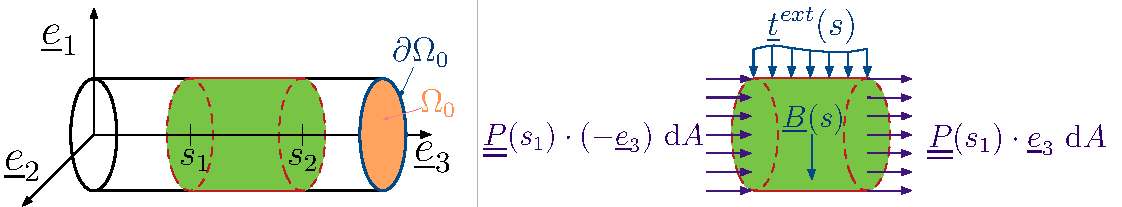
\includegraphics[width=22cm, keepaspectratio=true]{sections/cosserat_rods/images/Forces}
  \end{figure}

  \textbf{external forces}: body force $\underline{B}$ and external traction $\underline{t}^{ext}$
  
  \begin{displaymath}
    \begin{alignedat}{1}
      &\iiint_{\text{undeformed volume}} \underline{B} \dif V + \iint_{\text{lateral surface}} \underline{t}^{ext} \dif A = \\
      = &\int_{s_1}^{s_2} \Biggl( \iint_{\Omega_{0}(s)} \underline{B}(s) \dif A + \oint_{\partial \Omega_{0}(s)} \underline{t}^{ext}(s) \dif l \Biggr) \dif s =: \\
      =: & \int_{s_1}^{s_2} \underline{\hat{n}}(s) \dif s
    \end{alignedat}
  \end{displaymath}
  
  \vspace{0.5em}
  $\rightarrow$ distributed external load $\underline{\hat{n}}(s)$ (force per unit of undeformed length)
\end{frame}


%-------------------------------------------------------------------------------
\begin{frame}
  \frametitle{Balance of forces (part 2)}

  %\vspace{-0.5em}
  \begin{figure}
    \centering
    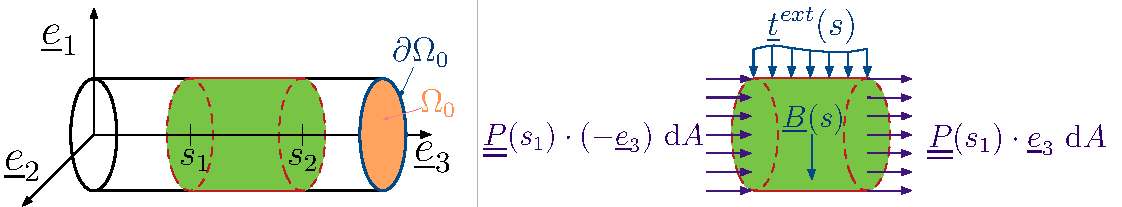
\includegraphics[width=22cm, keepaspectratio=true]{sections/cosserat_rods/images/Forces}
  \end{figure}

  %Material description: $\nabla_{\underline{X}} \cdot \doubleunderline{P} + \underline{B} = \rho_0 \cdot \underline{A}$

  \textbf{internal forces}
  
  \begin{displaymath}
    \begin{alignedat}{1}
      &\iint_{\Omega_0(s)} \doubleunderline{P} \cdot \underline{n} \dif A = \\
      = &\iint_{\Omega_0(s)} \doubleunderline{P}(X_1, X_2, s) \cdot \underline{e}_3 \dif X_1 \dif X_2 = \\
      =: \, &\underline{n}(s)
    \end{alignedat}
  \end{displaymath}
  
  \vspace{0.5em}
  $\rightarrow$ internal contact force $\underline{n}(s)$ (force per unit of undeformed length)
\end{frame}



%-------------------------------------------------------------------------------
\begin{frame}
  \frametitle{Balance of forces (part 3)}
  
  \begin{figure}
    \centering
    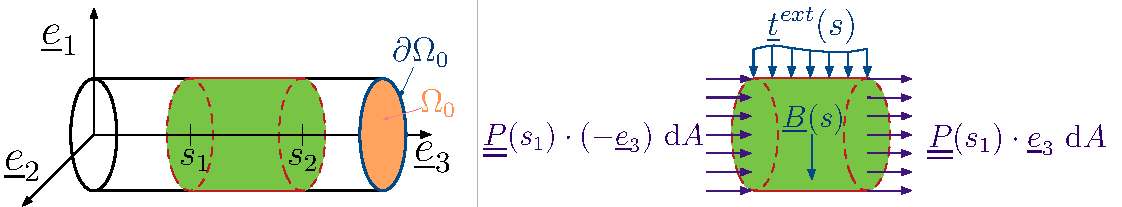
\includegraphics[width=22cm, keepaspectratio=true]{sections/cosserat_rods/images/Forces}
  \end{figure}
  
  \textbf{balance of forces} (statics)
  
  \begin{displaymath}
    \int_{s_1}^{s_2} \underline{\hat{n}}(s) \dif s + \underline{n}(s_2) - \underline{n}(s_1) =
    \int_{s_1}^{s_2} \underline{\hat{n}}(s) + \underline{n}^{\prime}(s) \dif s =
    \underline{0}
  \end{displaymath}
  
  since $s_1$ and $s_2$ are arbitrary cross sections we let $s_2 \to s_1$ \newline
  and obtain the \textbf{local force balance}
  \begin{displaymath}
    \underline{n}^{\prime}(s) + \underline{\hat{n}}(s) = \underline{0}
  \end{displaymath}
  \vspace{0.6em}
  
  \textbf{local balance of linear momentum} (dynamics)
  \begin{displaymath}
    \underline{n}^{\prime}(s) + \underline{\hat{n}}(s) = \rho_0 \, A \, \underline{\ddot{r}}(s)
  \end{displaymath}
\end{frame}


%-------------------------------------------------------------------------------
\begin{frame}
  \frametitle{Balance of moments (part 1)}
  
  we write the moment balance about the origin: $\underline{M} = \underline{x} \times \underline{F}$ \newline
  with $\underline{x}(X_1,X_2,s) = \underline{r}(s) + \bigl( \underline{x}(X_1,X_2,s) - \underline{r}(s) \bigr)$
  \vspace{0.5em}
  
  \textbf{moment due to external loads}
  \begin{displaymath}
    \begin{alignedat}{2}
      &\iiint_{\text{undeformed volume}} \underline{x} \times \underline{B} \dif V + &\\
       + &\iint_{\text{lateral surface}} \underline{x} \times \underline{t}^{ext} \dif A = &\\
      = &\int_{s_1}^{s_2} \Biggl( \underline{r}(s) \times \iint_{\Omega_{0}(s)} \underline{B}(s) \dif A \Biggr) \dif s +
        &\int_{s_1}^{s_2} \Biggl( \iint_{\Omega_{0}(s)} \bigl( \underline{x}(.,.,s) - \underline{r}(s) \bigr) \times \underline{B} \dif A \Biggr) \dif s + \\
        + &\int_{s_1}^{s_2} \Biggl( \underline{r}(s) \times \oint_{\partial \Omega_{0}(s)} \underline{t}^{ext}(s) \dif l \Biggr) \dif s +
        &\int_{s_1}^{s_2} \Biggl( \oint_{\partial \Omega_{0}(s)} \bigl( \underline{x}(.,.,s) - \underline{r}(s) \bigr) \times \underline{t}^{ext} \dif l \Biggr) \dif s =
    \end{alignedat}
  \end{displaymath}
\end{frame}



%-------------------------------------------------------------------------------
\begin{frame}
  \frametitle{Balance of moments (part 2)}
  % TODO use color to show which terms are equal
  \begin{displaymath}
    \begin{alignedat}{1}
      = &\int_{s_1}^{s_2} \Biggl( \underline{r}(s) \times \biggl( \iint_{\Omega_0} \underline{B}(s) \dif A + \oint_{\partial \Omega_{0}(s)} \underline{t}^{ext}(s) \dif l \biggr) \Biggr) \dif s + \\
        + &\int_{s_1}^{s_2} \biggl( \iint_{\Omega_{0}(s)} \bigl( \underline{x}(.,.,s) - \underline{r}(s) \bigr) \times \underline{B}(s) \dif A + \oint_{\partial \Omega_0} \bigl( \underline{x}(.,.,s) - \underline{r}(s) \bigr) \times \underline{t}^{ext}(s) \dif l \biggr) \dif s = \\
      =: &\int_{s_1}^{s_2} \underline{r}(s) \times \underline{\hat{n}}(s) \dif s +
        \int_{s_1}^{s_2} \underline{\hat{m}}(s) \dif s
    \end{alignedat}
  \end{displaymath}
\end{frame}


%-------------------------------------------------------------------------------
\begin{frame}
  \frametitle{Balance of moments (part 3)}
    % TODO use color to show which terms are equal
  \textbf{moment due to internal forces} % TODO tractions (also before with forces)
  \begin{displaymath}
    \begin{alignedat}{1}
      &\iint_{\Omega_0(s)} \underline{x}(X_1,X_2,s) \times \bigl( \doubleunderline{P}(X_1,X_2,s) \cdot \underline{e}_3 \bigr) \dif A = \\
      =&\iint_{\Omega_0(s)} \underline{r}(s) \times \bigl( \doubleunderline{P}(X_1,X_2,s) \cdot \underline{e}_3 \bigr) \dif X_1 \dif X_2 + \\
      + &\iint_{\Omega_0(s)} \bigl( \underline{x}(X_1,X_2,s) - \underline{r}(s) \bigr) \times \bigl( \doubleunderline{P}(X_1,X_2,s) \cdot \underline{e}_3 \bigr) \dif X_1 \dif X_2 = \\
      = \, &\underline{r}(s) \times \iint_{\Omega_0(s)} \doubleunderline{P}(X_1,X_2,s) \cdot \underline{e}_3 \dif X_1 \dif X_2 + \dots = \\
      =: \, &\underline{r}(s) \times \underline{n}(s) + \underline{m}(s)
    \end{alignedat}
  \end{displaymath}
\end{frame}


%-------------------------------------------------------------------------------
\begin{frame}
  \frametitle{Balance of moments (part 4)}
  
  \textbf{balance of moments} (statics)
  \begin{displaymath}
    \begin{alignedat}{1}
      &\int_{s_1}^{s_2} \bigl( \underline{r}(s) \times \underline{\hat{n}}(s) + \underline{\hat{m}}(s)\bigr) \dif s + \\ 
      &+ \bigl( \underline{r}(s_2) \times \underline{n}(s_2) + \underline{m}(s_2) \bigr)
         - \bigl( \underline{r}(s_1) \times \underline{n}(s_1) + \underline{m}(s_1) \bigr) = \\
      &= \int_{s_1}^{s_2} \Bigl( \bigl( \cancel{\underline{r}(s) \times \underline{\hat{n}}(s)} + \underline{\hat{m}}(s) \bigr) + \bigl( \underline{r}^{\prime}(s) \times \underline{n}(s) + \cancel{\underline{r}(s) \times \underline{n}^{\prime}(s)} + \underline{m}^{\prime}(s) \bigr) \Bigr) \dif s = \\
      &= \int_{s_1}^{s_2} \bigl( \underline{\hat{m}}(s) + \underline{r}^{\prime}(s) \times \underline{n}(s) + \underline{m}^{\prime}(s) \bigr) \dif s
    \end{alignedat}
  \end{displaymath}
  % Note: terms canceled because of force balance
  
  since $s_1$ and $s_2$ are arbitrary cross sections we let $s_2 \to s_1$ \newline
  and obtain the \textbf{local moment balance}
  \begin{displaymath}
    \underline{m}^{\prime}(s) + \underline{r}^{\prime}(s) \times \underline{n}(s) + \underline{\hat{m}}(s) = \underline{0}
  \end{displaymath}

%  \begin{displaymath}
%    \underline{m}^{\prime}(s) +
%    \underline{r}^{\prime}(s) \times \underline{n}(s) +
%    \underline{\hat{m}}(s) =
%    \rho_0 \cdot
%    \bar{
%      \bigl( \dot{\doubleunderline{I} \cdot \underline{\omega}} \bigr)
%    } =
%    \underline{0}
%  \end{displaymath}
    % TODO dynamics, widebar
\end{frame}


%-------------------------------------------------------------------------------

\begin{frame}
  \frametitle{Review of balance equations (statics)}
  
  \textbf{force balance} (3 equations)
  \begin{displaymath}
    \underline{n}^{\prime}(s) + \underline{\hat{n}}(s) = \underline{0}
  \end{displaymath}
  
  \textbf{moment balance} (3 equations)
  \begin{displaymath}
    \underline{m}^{\prime}(s) + \underline{r}^{\prime}(s) \times \underline{n}(s) + \underline{\hat{m}}(s) = \underline{0}
  \end{displaymath}
  
  \vspace{1em}
  we have \textbf{6 kinematic unknowns}, $\underline{r}(s)$ and $\doubleunderline{R}(s)$ with 3 unknowns each
  
  \vspace{0.3em}
  and we have \textbf{6 kinetic unknowns}
  \begin{displaymath}
    \begin{alignedat}{1}
      &\underline{n}(s) = \iint_{\Omega_0(s)} \doubleunderline{P}(X_1, X_2, s) \cdot \underline{e}_3 \dif X_1 \dif X_2 \\
      &\underline{m}(s) = \iint_{\Omega_0(s)} \bigl( \underline{x}(X_1,X_2,s) - \underline{r}(s) \bigr) \times \bigl( \doubleunderline{P}(X_1,X_2,s) \cdot \underline{e}_3 \bigr) \dif X_1 \dif X_2
    \end{alignedat}
  \end{displaymath}
  
  \vspace{0.3em}
  to close the system we need a relationship between the kinematic and the kinetic quatities
\end{frame}


%===============================================================================
\subsection{Constitutive laws}

%-------------------------------------------------------------------------------
\begin{frame}
  \frametitle{Motivation of constitutive law}

  let's recall the \textbf{constrained deformation map} (without warping)
  \begin{displaymath}
    \underline{x}(X_1,X_2,s) = \underline{f}(X_1,X_2,s) = \underline{r}(s) + X_{\alpha} \, \underline{d}_{\alpha} = \underline{r}(s) + \doubleunderline{R}(s) \cdot ( X_{\alpha} \, \underline{e}_{\alpha} )
  \end{displaymath}
  
  we compute the \textbf{deformation gradient} and obtain
  % TODO computation of F in more detail?
  \begin{displaymath}
    \begin{alignedat}{1}
      \doubleunderline{F}(X_1,X_2,s) &= \underline{r}^{\prime}(s) \otimes \underline{e}_3 + \doubleunderline{R}(s) \: \underline{e}_{\alpha} \otimes \underline{e}_{\alpha} + \doubleunderline{R}^{\prime}(s) \: X_{\alpha} \underline{e}_{\alpha} \otimes \underline{e}_3 = \\
      &= \doubleunderline{R}(s) \biggl( \doubleunderline{R}^{\mathrm{T}}(s) \, \underline{r}^{\prime}(s) \otimes \underline{e}_3 + \underline{e}_{\alpha} \otimes \underline{e}_{\alpha} + \doubleunderline{R}^{\mathrm{T}}(s) \, \doubleunderline{R}^{\prime}(s) \, X_{\alpha} \underline{e}_{\alpha} \otimes \underline{e}_3 \biggr)
    \end{alignedat}
  \end{displaymath}
  
  \vspace{1em}
  we then obtain an expression of the form
  \begin{displaymath}
    \doubleunderline{P}(X_1,X_2,s) = \mathop{\mathrm{function}}\bigl( \doubleunderline{F}(X_1,X_2,s) \bigr) \, ,
  \end{displaymath}
  
  \vspace{0.4em}
  %which leads us to the constitutive law ...
  from the 3-dimensional constitutive law of the material
\end{frame}



%-------------------------------------------------------------------------------
\begin{frame}
  \frametitle{Example with constrained deformation map: stretching of a bar}
  
  \vspace{-1em}
  \begin{multicols}{2}
    \noindent
    \begin{figure}
      \centering
      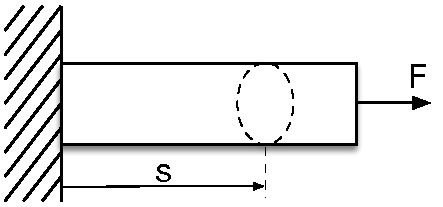
\includegraphics[width=8cm, keepaspectratio=true]{sections/cosserat_rods/images/ExampleConstrainedMapStretchingBar}
    \end{figure}
    
    we have the \textbf{deformed configuration}
    \begin{displaymath}
      \begin{alignedat}{1}
        \underline{r}(s) &= \lambda \, s \, \underline{e}_3 \quad \text{with } \lambda \in \mathbb{R}^{+} \\
        \doubleunderline{R}(s) &= \doubleunderline{I} \\
      \end{alignedat}
    \end{displaymath}
  \end{multicols}
  
  \vspace{-0.5em}
  therefore the \textbf{deformation map} is
  \begin{displaymath}
    \underline{x}(X_1,X_2,s) \underline{x}(s) = \lambda \, s \, \underline{e}_3 + \doubleunderline{I} \cdot (X_{\alpha} \, \underline{e}_{\alpha})
  \end{displaymath}
  
  and its \textbf{deformation gradient} is given by
  \begin{displaymath}
    \doubleunderline{F}(X_1,X_2,s) = \doubleunderline{F}(s) = \lambda \, \underline{e_3} \otimes \underline{e_3} + \underline{e}_{\alpha} \otimes \underline{e}_{\alpha} = (\lambda - 1) \underline{e}_3 \otimes \underline{e}_3 + \doubleunderline{I}  
  \end{displaymath}
  
  but the \textbf{axial force}
  \begin{displaymath}
    \begin{alignedat}{1}
      \underline{n}(s) &= \iint_{\Omega_0(s)} \doubleunderline{P}(X_1, X_2, s) \cdot \underline{e}_3 \dif X_1 \dif X_2 \\
      &\neq E \, A \, (\lambda - 1)
    \end{alignedat}
  \end{displaymath}
  because the deformation map violates the traction-free boundary condition \newline
  $\rightarrow$ the cross section must be able to shrink when the bar is stretched!
\end{frame}


%-------------------------------------------------------------------------------
\begin{frame}
  \frametitle{Constitutive equation for a hyperelastic rod}
  
  note: hyperelasticity refers to a reversible deformation process; \newline
  therefore it can be described by a potential function
  
  \vspace{0.7em}
  in order to derive constitutive laws from theory, \newline
  we will use functions that are potentials of internal energy ... 
  
  \vspace{1.5em}
  \textbf{strain energy per unit of undeformed length}
  \begin{displaymath}
    \phi = \phi \bigl( \underline{r}(s),\doubleunderline{R}(s),\underline{r}^{\prime}(s),\doubleunderline{R}^{\prime}(s) \bigr)
  \end{displaymath}
  
  \vspace{1.5em}
  \textbf{strain energy per unit of undeformed volume}
  \begin{displaymath}
    W \bigl( \cancel{\underline{f}(s)}, \doubleunderline{F}(s), \cancel{\nabla \doubleunderline{F}(s)} \bigr) = W \bigl( \doubleunderline{F}(s) \bigr)
  \end{displaymath}

  \vspace{0.1em}
  \begin{itemize}
    \item $\underline{f}(s)$ canceled because of principle of frame indifference
    \item $\nabla \doubleunderline{F}(s)$ canceled because we will not consider higher order derivatives of the deformation map in classical elasticity (compared to higher gradient elasticity theory)
    % discontinuities at interfaces in the material 
  \end{itemize}
\end{frame}


%-------------------------------------------------------------------------------
\begin{frame}
  \frametitle{Principle of material frame-indifference (part 1)}

  \vspace{-0.5em}
  \begin{itemize}
    \item  constitutive laws should be invariant with regard to the external frame of reference, \newline i.e. the coordinate system ($\rightarrow$ observer objectivity)
    \item $\Rightarrow$ rigid body motions do not affect the internally stored energy in the system, \newline \null \quad (i.e. the mechanical/deformation energy)
    \item $\rightarrow$ we want to identify a set of strain measures which is invariant to rigid body motions!
  \end{itemize}
  
  \vspace{0.3em}
  to that end we set up a simple \textbf{thought experiment}
  \begin{itemize}
    \item perform two rigid body motions: one rotation followed by one translation
    \item equate the internal mechanical energy potentials: $\eval[1]{\phi}_{\alpha} = \eval[1]{\phi}_{\beta} = \eval[1]{\phi}_{\gamma}$
  \end{itemize}
  
  \vspace{-1.4em}
  \begin{figure}
    \centering
    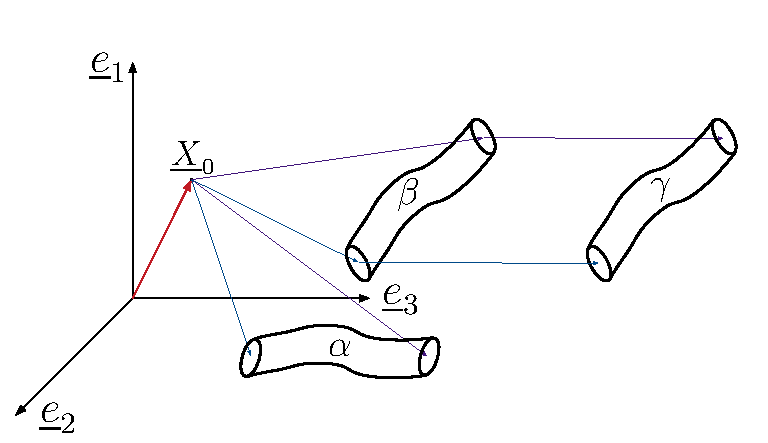
\includegraphics[width=13cm, keepaspectratio=true]{sections/cosserat_rods/images/FrameIndifferenceExperiment}
  \end{figure}  
\end{frame}


%-------------------------------------------------------------------------------
\begin{frame}
  \frametitle{Principle of material frame-indifference (part 2)}
  % TODO split slide
  \vspace{-0.6em}
  \begin{enumerate}
    \item initial configuration $\alpha$
      \begin{itemize}
        \item centerline given by $\underline{r}^{\alpha}(s)$
        \item cross section orientation given by $\doubleunderline{R}^{\alpha}(s)$
        \item energy potential given by $\eval[1]{\phi}_{\beta}(s) = \phi \bigl( \underline{r}^{\alpha}{\alpha}(s) , \, \doubleunderline{R}^{\alpha}(s) , \, \underline{r}^{\alpha \prime}(s) , \, \doubleunderline{R}^{\alpha \prime}(s) \bigr)$
      \end{itemize}
      
    \item configuration $\beta$ after rigid body rotation by $\doubleunderline{Q}$ about $\underline{X}_0$ 
      (arbitrary $\doubleunderline{Q} \in SO(3)$ , $\underline{X}_0 \in \mathbb{R}^3$)
      \begin{itemize}
        \item $\underline{r}^{\beta}(s) = \underline{X}_0 + \doubleunderline{Q} \left( \underline{r}^{\alpha}(s) - \underline{X}_0 \right) \quad \Rightarrow \quad \underline{r}^{\beta \prime}(s) = \doubleunderline{Q} \, \underline{r}^{\alpha \prime}(s)$ \newline
          \null \quad (shift coordinate system s.t. rotation's fix-point $\hat{=}$ origin; rotate; undo shift)
        \item $\doubleunderline{R}^{\beta}(s) = \doubleunderline{Q} \, \doubleunderline{R}^{\alpha}(s) \quad \Rightarrow \quad \doubleunderline{R}^{\beta \prime}(s) = \doubleunderline{Q} \, \doubleunderline{R}^{\alpha \prime}(s)$
        \item $\eval[1]{\phi}_{\beta}(s) = \phi \bigl( \underline{X}_0 + \doubleunderline{Q} \left( \underline{r}^{\alpha}(s) - \underline{X}_0 \right) , \, \doubleunderline{Q} \, \doubleunderline{R}^{\alpha}(s) , \, \doubleunderline{Q} \, \underline{r}^{\alpha \prime}(s) , \, \doubleunderline{Q} \, \doubleunderline{R}^{\alpha \prime}(s) \bigr)$
      \end{itemize}
      
    \item configuration $\gamma$ after rigid body translation by $\underline{t}$ (arbitrary $\underline{t} \in \mathbb{R}^3$)
      \begin{itemize}
        \item $\underline{r}^{\gamma}(s) = \underline{X}_0 + \doubleunderline{Q} \left( \underline{r}^{\alpha}(s) - \underline{X}_0 \right) + \underline{t} \quad \Rightarrow \quad \underline{r}^{\gamma \prime}(s) = \underline{r}^{\beta \prime}(s) = \doubleunderline{Q} \,\underline{r}^{\alpha \prime}(s)$
        \item $\doubleunderline{R}^{\gamma}(s) = \doubleunderline{I} \, \doubleunderline{R}^{\beta}(s) = \doubleunderline{Q} \, \doubleunderline{R}^{\alpha}(s) \quad \Rightarrow \quad \doubleunderline{R}^{\gamma \prime}(s) = \doubleunderline{R}^{\beta \prime}(s) = \doubleunderline{Q} \, \doubleunderline{R}^{\alpha \prime}(s)$
        \item $\eval[1]{\phi}_{\gamma}(s) = \phi \bigl( \underline{X}_0 + \doubleunderline{Q} \left( \underline{r}^{\alpha}(s) - \underline{X}_0 \right) + \underline{t} , \, \doubleunderline{Q} \, \doubleunderline{R}^{\alpha}(s) , \, \doubleunderline{Q} \,\underline{r}^{\alpha \prime}(s) , \, \doubleunderline{Q} \, \doubleunderline{R}^{\alpha \prime}(s) \bigr)$
      \end{itemize}
  \end{enumerate}
\end{frame}



%-------------------------------------------------------------------------------
\begin{frame}
  \frametitle{Principle of material frame-indifference (part 3)}
  
  comparing $\eval[1]{\phi}_{\beta}(s) \overset{!}{=} \eval[1]{\phi}_{\gamma}(s)$ gives
  \begin{displaymath}
    \begin{alignedat}{4}
      \phi \bigl(
        &\underline{X}_0 + \doubleunderline{Q} \left( \underline{r}^{\alpha}(s) - \underline{X}_0 \right) , \,
        &\doubleunderline{Q} \, \doubleunderline{R}^{\alpha}(s) , \,
        &\doubleunderline{Q} \, \underline{r}^{\alpha \prime}(s) , \,
        &\doubleunderline{Q} \, \doubleunderline{R}^{\alpha \prime}(s)
      \bigr) = \\
      \phi \bigl(
        &\underline{X}_0 + \doubleunderline{Q} \left( \underline{r}^{\alpha}(s) - \underline{X}_0 \right) + \underline{t} , \,
        &\doubleunderline{Q} \, \doubleunderline{R}^{\alpha}(s) , \,
        &\doubleunderline{Q} \, \underline{r}^{\alpha \prime}(s) , \,
        &\doubleunderline{Q} \, \doubleunderline{R}^{\alpha \prime}(s)
      \bigr) \Rightarrow
    \end{alignedat}
  \end{displaymath}
  $\Rightarrow \phi$ is independent of $\underline{r}(s)$, i.e. the first argument can be omitted
  
  \vspace{1em}
  without loss of generality we can set the arbitrarily chosen rotation matrix $\doubleunderline{Q} := \doubleunderline{R}^{\mathrm{T}}$
  \begin{displaymath}
    \phi(s) = \phi \bigl(
        . , \,
        \doubleunderline{R}^{\mathrm{T}}(s) \, \doubleunderline{R}(s) , \,
        \doubleunderline{R}^{\mathrm{T}}(s) \, \underline{r}^{\prime}(s) , \,
        \doubleunderline{R}^{\mathrm{T}}(s) \, \doubleunderline{R}^{\prime}(s)
      \bigr)
  \end{displaymath}
  
  \vspace{1em}
  we define a new version of $\phi$ that depends only on the invariants
  \begin{displaymath}
    \psi(s) := \psi \bigl(
      \doubleunderline{R}^{\mathrm{T}}(s) \, \underline{r}^{\prime}(s) , \,
      \doubleunderline{R}^{\mathrm{T}}(s) \, \doubleunderline{R}^{\prime}(s)
    \bigr)
  \end{displaymath}  
\end{frame}


%-------------------------------------------------------------------------------
\begin{frame}
  \frametitle{Invariant strain measures (part 1)}
  
  
  we can verify that $\doubleunderline{R}^{\mathrm{T}} \, \underline{r}^{\prime}$ and $\doubleunderline{R}^{\mathrm{T}} \, \doubleunderline{R}^{\prime}$ are truly invariant strain measures
  
  \vspace{1em}
  we get
  \begin{displaymath}
    \doubleunderline{R}^{\gamma \mathrm{T}} \, \underline{r}^{\gamma \prime} =
    \bigl( \doubleunderline{Q} \, \doubleunderline{R}^{\alpha} \bigr)^{\mathrm{T}} \, \bigl( \doubleunderline{Q} \, \underline{r}^{\alpha \prime} \bigr) =
    \bigl( \doubleunderline{R}^{\alpha \mathrm{T}} \, \doubleunderline{Q}^{\mathrm{T}} \bigr) \, \bigl( \doubleunderline{Q} \, \underline{r}^{\alpha \prime} \bigr) =
    \doubleunderline{R}^{\alpha \mathrm{T}} \, \underline{r}^{\alpha \prime}
  \end{displaymath}
  and
  \begin{displaymath}
    \doubleunderline{R}^{\gamma \mathrm{T}} \, \doubleunderline{R}^{\gamma \prime} =
    \bigl( \doubleunderline{Q} \, \doubleunderline{R}^{\alpha} \bigr)^{\mathrm{T}} \, \bigl( \doubleunderline{Q} \, \doubleunderline{R}^{\alpha \prime} \bigr) =
    \bigl( \doubleunderline{R}^{\alpha \mathrm{T}} \, \doubleunderline{Q}^{\mathrm{T}} \bigr) \, \bigl( \doubleunderline{Q} \, \doubleunderline{R}^{\alpha \prime} \bigr) =
    \doubleunderline{R}^{\alpha \mathrm{T}} \, \doubleunderline{R}^{\alpha \prime}
  \end{displaymath}
\end{frame}


%-------------------------------------------------------------------------------
\begin{frame}
  \frametitle{Invariant strain measures (part 2)}
  we define $\underline{v}$ as the shorthand for the first invariant
  \begin{displaymath}
    \underline{v} =
    \begin{bmatrix} v_1 \\ v_2 \\ v_3 \end{bmatrix} = 
    v_i \, \underline{e}_i :=
    \doubleunderline{R}^{\mathrm{T}} \, \underline{r}^{\prime}
    \quad \Rightarrow \quad
    \underline{r}^{\prime} =
    \doubleunderline{R} \, \underline{v} =
    v_i \, \doubleunderline{R} \, \underline{e}_i =
    v_i \, \underline{d}_i
  \end{displaymath}
  
  and from orthogonality of the director basis ($\underline{d}_i \cdot \underline{d}_j = \delta_{ij}$) it follows that $v_i = \underline{r}^{\prime} \cdot \underline{d}_i$
  
  \vspace{0.3em}
  $\rightarrow \underline{v} = \doubleunderline{R}^{\mathrm{T}} \, \underline{r}^{\prime}$ is the centerline tangent vector resolved in the local director basis!
  
  \vspace{1em}
  more specifically we have ...
  \begin{itemize}
    \item $v_1 = \underline{r}^{\prime} \, \underline{d}_1$ : rate of transverse shift $\hat{=}$ shear along $\underline{d}_1$
    \item $v_2 = \underline{r}^{\prime} \, \underline{d}_2$ : shear along $\underline{d}_2$
    \item $v_3 = \underline{r}^{\prime} \, \underline{d}_3$ : rate of axial shift $\hat{=}$ axial stretch 
  \end{itemize}
  % TODO make a figure
\end{frame}


%-------------------------------------------------------------------------------
\begin{frame}
  \frametitle{Invariant strain measures (part 3)}
  
  we define $\doubleunderline{K}$ as the shorthand for the second invariant
  \begin{displaymath}
    \doubleunderline{K} =
    K_{ij} \, \underline{e}_i \otimes \underline{e}_j :=
    \doubleunderline{R}^{\mathrm{T}} \, \doubleunderline{R}^{\prime}
  \end{displaymath}
  
  \vspace{0.5em}
  \textbf{proof} that $\doubleunderline{K}$ is \textit{skew-symmetric} ($K_{ij} = -K_{ji}$)
  \begin{displaymath}
    \doubleunderline{R}^{\mathrm{T}} \, \doubleunderline{R} = \doubleunderline{I}
    \quad \Rightarrow \quad
    \doubleunderline{R}^{\mathrm{T}} \, \doubleunderline{R}^{\prime} + \doubleunderline{R}^{\prime \mathrm{T}} \, \doubleunderline{R} = \doubleunderline{0}
    \quad \Rightarrow \quad
    \doubleunderline{K} = -\doubleunderline{K}^{\mathrm{T}}
  \end{displaymath}
  
  \vspace{0.5em}
  we therefore can write
  \begin{displaymath}
    \doubleunderline{K} = 
    \begin{bmatrix}
       0   & -k_3 &  k_2 \\
       k_3 &  0   & -k_1 \\
      -k_2 &  k_1 &  0
    \end{bmatrix}
  \end{displaymath}
  \vspace{0.5em}
  and we recall that $\doubleunderline{K} \, \underline{a} = \underline{k} \times \underline{a} \: \forall \underline{a} \in \mathbb{R}^3$ with $\underline{k} = \axial(\doubleunderline{K}) = k_i \, \underline{e}_i$
  
  \vspace{1em}
  $\rightarrow$ with $\left( \underline{v} , \, \underline{k} \right)$ we have the 6 strain measures given in the frame of the director basis! \newline
  $\rightarrow$ $\psi = \psi \bigl( \underline{v} , \, \doubleunderline{K} \bigr) =: \hat{\psi} \bigl( \underline{v} , \, \underline{k} \bigr)$ (for easy notation we will drop the $\hat{.}$ in the sequel)
\end{frame}


%-------------------------------------------------------------------------------
\begin{frame}
  \frametitle{Invariant strain measures (part 4)}

  to better understand the physical meaning of $\underline{k}$ we have a look at two examples ...
  
  \vspace{0.5em}
  \textbf{pure twisting of a rod}
  \vspace{-1em}
  \begin{multicols}{2}
    \noindent
    
    \begin{figure}
      \centering
      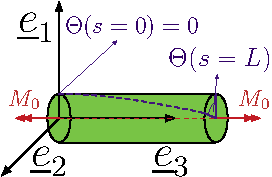
\includegraphics[width=10cm, keepaspectratio=true]{sections/cosserat_rods/images/PureTwistingExample}
    \end{figure}

    \begin{itemize}
      \item rotation of cross sections around $\underline{e}_3$-axis
      \item angle of rotation for the cross section at $s$ given by $\Theta(s) = \Theta^{\prime} \cdot s$ \newline
        with $\Theta^{\prime} = const.$ because external moments act only at $s=0$ and $s=L$
    \end{itemize}
    \vspace{0.1em}
    \begin{displaymath}
      \underline{r}(s) = s \cdot \underline{e}_3 
      \: \Rightarrow \:
      \underline{r}^{\prime}(s) = \underline{e}_3
    \end{displaymath}
    \begin{displaymath}
      \: \Rightarrow \:
      \underline{v} = \doubleunderline{R}^{\mathrm{T}} \, \underline{r}^{\prime} =
      \begin{bmatrix}
        0 & 0 & 1
      \end{bmatrix}^{\mathrm{T}}
      \: \Rightarrow \:
      v_3 = 1
    \end{displaymath}
%    \begin{displaymath}
%      \underline{r}(s) = s \cdot \underline{e}_3 
%      \: \Rightarrow \:
%      \underline{r}^{\prime}(s) = \underline{e}_3
%      \: \Rightarrow \:
%      \underline{v} = \doubleunderline{R}^{\mathrm{T}} \, \underline{r}^{\prime} =
%      \begin{bmatrix}
%        0 & 0 & 1
%      \end{bmatrix}^{\mathrm{T}}
%      \: \Rightarrow \:
%      v_3 = 1
%    \end{displaymath}
  \end{multicols}
  \vspace{-1.2em}
  \begin{displaymath}
    \doubleunderline{R}(s) =
    \begin{bmatrix}
      +\cos(\Theta(s)) & -\sin(\Theta(s)) & 0 \\
      +\sin(\Theta(s)) & +\cos(\Theta(s)) & 0 \\
      0 & 0 & 1
    \end{bmatrix}
    \: \Rightarrow \:
    \doubleunderline{R}^{\prime}(s) =
    \Theta^{\prime} \cdot
    \begin{bmatrix}
      -\sin(\Theta(s)) & -\cos(\Theta(s)) & 0 \\
      +\cos(\Theta(s)) & -\sin(\Theta(s)) & 0 \\
      0 & 0 & 0
    \end{bmatrix}
  \end{displaymath}
    
  \begin{displaymath}
    \doubleunderline{K}(s) =
    \doubleunderline{R}^{\mathrm{T}}(s) \, \doubleunderline{R}^{\prime}(s) =
    \begin{bmatrix}
      0 & -\Theta^{\prime} & 0 \\
      +\Theta^{\prime} & 0 & 0 \\
      0 & 0 & 0
    \end{bmatrix}
    \: \Rightarrow \:
    \underline{k} =
    \begin{bmatrix}
      0 \\ 0 \\ \Theta^{\prime}
    \end{bmatrix}
    \: \Rightarrow \:
    k_3 = \Theta^{\prime}
  \end{displaymath}
\end{frame}

%-------------------------------------------------------------------------------
\begin{frame}
  \frametitle{Invariant strain measures (part 5)}

  \textbf{pure bending of a rod}
  \begin{multicols}{2}
    \noindent
    \begin{figure}
      \centering
      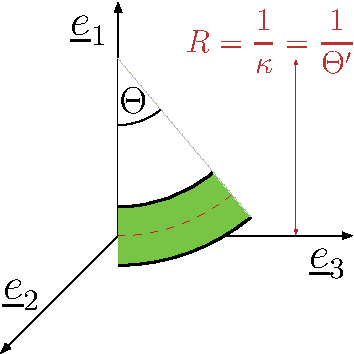
\includegraphics[width=8cm, keepaspectratio=true]{sections/cosserat_rods/images/PureBendingExample}
    \end{figure}
    
    \begin{itemize}
      \item rotation of cross sections around $\underline{e}_2$-axis
      \item angle of rotation for the cross section at $s$ given by $\Theta(s) = \Theta^{\prime} \cdot s = \kappa \cdot s$\newline
        with $\Theta^{\prime} = \kappa = const.$ because external moments act only at $s=0$ and $s=L$
    \end{itemize}
    \vspace{0.1em}
    \begin{displaymath}
      \underline{r}(s) = s \cdot \underline{e}_3 
      \: \Rightarrow \:
      \underline{r}^{\prime}(s) = \underline{e}_3
    \end{displaymath}
    \begin{displaymath}
      \: \Rightarrow \:
      \underline{v} = \doubleunderline{R}^{\mathrm{T}} \, \underline{r}^{\prime} =
      \begin{bmatrix}
        0 & 0 & 1
      \end{bmatrix}^{\mathrm{T}}
      \: \Rightarrow \:
      v_3 = 1
    \end{displaymath}
    \vspace{0.6em}
  \end{multicols}  

  \vspace{-2em}
  \begin{displaymath}
    \doubleunderline{R}(s) =
    \begin{bmatrix}
      +\cos(\Theta(s)) & 0 & +\sin(\Theta(s))\\
      0 & 1 & 0 \\
      -\sin(\Theta(s)) & 0 & +\cos(\Theta(s))
    \end{bmatrix}
    \: \Rightarrow \:
    \doubleunderline{R}^{\prime}(s) =
    \Theta^{\prime} \cdot
    \begin{bmatrix}
      -\sin(\Theta(s)) & 0 & +\cos(\Theta(s))\\
      0 & 0 & 0 \\
      -\cos(\Theta(s)) & 0 & -\sin(\Theta(s))
    \end{bmatrix}
  \end{displaymath}
  
  \begin{displaymath}
    \doubleunderline{K}(s) =
    \doubleunderline{R}^{\mathrm{T}}(s) \, \doubleunderline{R}^{\prime}(s) =
    \begin{bmatrix}
      0 & 0 & +\Theta^{\prime} \\
      0 & 0 & 0 \\
      -\Theta^{\prime} & 0 & 0
    \end{bmatrix}
    \: \Rightarrow \:
    \underline{k} =
    \begin{bmatrix}
      0 \\ \Theta^{\prime} \\ 0
    \end{bmatrix}
    \: \Rightarrow \:
    k_2 = \Theta^{\prime}
  \end{displaymath}
\end{frame}

%-------------------------------------------------------------------------------
\begin{frame}
  \frametitle{Recap of what we have so far}
  \textbf{balance equations}
  \begin{displaymath}
    \underline{n}^{\prime} + \underline{\hat{n}} = \underline{0}
    \quad \text{ and } \quad
    \underline{m}^{\prime} + \underline{r}^{\prime} \times \underline{n} + \underline{\hat{m}} = \underline{0}
  \end{displaymath}
  
  \vspace{2em}
  \textbf{deformation energy per unit of undeformed length}
  \begin{displaymath}
    \psi \bigl( \doubleunderline{R}^{\mathrm{T}} \, \underline{r}^{\prime} , \, \doubleunderline{R}^{\mathrm{T}} \, \doubleunderline{R}^{\prime} \bigr) =
    \psi \bigl( \underline{v} , \, \doubleunderline{K} \bigr) =
    \psi \bigl( \underline{v} , \, \underline{k} \bigr)  \end{displaymath}
\end{frame}


%-------------------------------------------------------------------------------
\begin{frame}
  \frametitle{Minimum potential energy method (part 1)}
  
  we consider a system consisting of a beam with and an external load $P$ at $s=L$
  
  \vspace{-0.3em}
  \begin{figure}
    \centering
    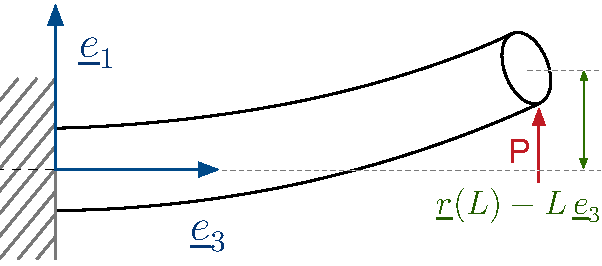
\includegraphics[width=14cm, keepaspectratio=true]{sections/cosserat_rods/images/MinimumPotentialEnergyMethodExample}
  \end{figure}
  
  the \textbf{total energy of the closed system} is given by
  \begin{displaymath}
    \Pi \bigl( \underline{r}, \, \doubleunderline{R} \bigr) =
    \int_0^L \psi \bigl( \underline{v} , \, \underline{k} \bigr) \dif s - P \, \underline{e}_1 \cdot \underline{r}(L)
  \end{displaymath}
  note regarding minus sign: load performs work on the beam, \newline
  thereby lowering the load's potential and also the potential of the closed system
  
  \vspace{0.3em}
  $\rightarrow$ we now want to identify the conditions for a minimum of $\Pi$
\end{frame}


%-------------------------------------------------------------------------------
\begin{frame}
  \frametitle{Minimum potential energy method (part 2)}
  
  \textbf{perturbed versions of $\underline{r}$ and $\doubleunderline{R}$}
  \begin{displaymath}
    \underline{r}_{\epsilon}(s) = \underline{r}(s) + \epsilon \cdot \delta \underline{r}(s)
  \end{displaymath}
  \vspace{-0.5em}
  \begin{displaymath}
    \doubleunderline{R}_{\epsilon}(s) = \underbrace{\xcancel{\doubleunderline{R}(s) + \epsilon \cdot \delta \doubleunderline{R}(s)}}_{\notin SO(3)} = \underbrace{\exp \bigl( \epsilon \cdot \delta \doubleunderline{\Theta}(s) \bigr)}_{\in SO(3)} \, \doubleunderline{R}(s)
    \quad \text{ with } \quad
    \delta \underline{\Theta} := \axial \bigl( \delta \doubleunderline{\Theta} \bigr)
  \end{displaymath}
  
  \vspace{0.6em}
  \textbf{perturbed version of total energy}
  \begin{displaymath}
    \Pi \bigl( \underline{r}_{\epsilon}, \, \doubleunderline{R}_{\epsilon} \bigr) =
    \int_0^L \psi \bigl( \underline{v}_{\epsilon} , \, \underline{k}_{\epsilon} \bigr) \dif s - P \, \underline{e}_1 \cdot \underline{r}_{\epsilon}(L) \overset{!}{=}
    \Pi \bigl( \underline{r}, \, \doubleunderline{R} \bigr) + \epsilon \cdot \delta \Pi \bigl( \underline{r}, \, \doubleunderline{R} \bigr) + \mathcal{o}(\epsilon)
  \end{displaymath}
  
  \vspace{0.6em}
  \textbf{first variation of total energy}
  \begin{displaymath}
    \delta \Pi = \pd{\Pi}{\epsilon} \sVert[3]_{\epsilon=0} =
    \int_0^L \biggl(
    \pd{\psi}{\underline{v}}(s) \cdot \underbrace{ \pd{\underline{v}_{\epsilon}}{\epsilon}(s) \sVert[2]_{\epsilon=0} }_{\delta \underline{v}(s)} +
    \pd{\psi}{\underline{k}}(s) \cdot \underbrace{ \pd{\underline{k}_{\epsilon}}{\epsilon}(s)\sVert[2]_{\epsilon=0} }_{\delta \underline{k}(s)}
    \biggr) \dif s
    - P \, \underline{e}_1 \cdot \pd{\underline{r}_{\epsilon}}{\epsilon}(L) \sVert[3]_{\epsilon=0}
  \end{displaymath}
  
  in the sequel we will work on the terms $\delta \underline{v}(s)$ and $\delta \underline{k}(s)$
\end{frame}


%-------------------------------------------------------------------------------
\begin{frame}
  \frametitle{Minimum potential energy method (part 3)}
  
  \textbf{perturbed version of $\underline{v}$}
  \begin{displaymath}
    \underline{v}_{\epsilon}(s) =
    \doubleunderline{R}_{\epsilon}^{\mathrm{T}}(s) \cdot \underline{r}_{\epsilon}^{\prime}(s) =
    \doubleunderline{R}^{\mathrm{T}}(s) \cdot \biggl( \exp \bigl( \epsilon \cdot \delta \doubleunderline{\Theta}(s) \bigr) \biggr)^{\mathrm{T}} \cdot \bigl( \underline{r}^{\prime}(s) + \epsilon \cdot \delta \underline{r}^{\prime}(s) \bigr)
  \end{displaymath}
  
  \vspace{0.5em}
  \textbf{first variation of $\underline{v}$}
  \begin{displaymath}
    \delta \underline{v}(s) = 
    \pd{\underline{v}_{\epsilon}}{\epsilon}(s) \sVert[3]_{\epsilon=0} =
    \doubleunderline{R}^{\mathrm{T}}(s) \cdot
    \pd{}{\epsilon} \biggl( \exp \bigl( \epsilon \cdot \delta \doubleunderline{\Theta}(s) \bigr) \biggr)^{\mathrm{T}} \sVert[3]_{\epsilon=0}
     \cdot \underline{r}^{\prime}(s) +
     \doubleunderline{R}^{\mathrm{T}}(s) \cdot \delta \underline{r}^{\prime}(s)
  \end{displaymath}
  
  \vspace{0.5em}
  \begin{displaymath}
    \pd{}{\epsilon} \biggl( \exp \bigl( \epsilon \cdot \delta \doubleunderline{\Theta}(s) \bigr) \biggr)^{\mathrm{T}} \sVert[3]_{\epsilon=0} =
    \pd{}{\epsilon} \biggl( \doubleunderline{I} + \epsilon \cdot \delta \doubleunderline{\Theta} + \frac{\epsilon^2}{2} \cdot \delta \doubleunderline{\Theta}^2 + \dots \biggr)^{\mathrm{T}} \sVert[3]_{\epsilon=0} =
    \bigl( \delta \doubleunderline{\Theta} \bigr)^{\mathrm{T}} = -\delta \doubleunderline{\Theta} 
  \end{displaymath}
  
  \vspace{0.5em}
  \begin{displaymath}
    \Rightarrow
    \delta \underline{v}(s) =
    \doubleunderline{R}^{\mathrm{T}}(s) \cdot
    \bigl( - \delta \doubleunderline{\Theta}(s) \cdot \underline{r}^{\prime}(s) + \delta \underline{r}^{\prime}(s) \bigr)
  \end{displaymath}
\end{frame}



%-------------------------------------------------------------------------------
\begin{frame}
  \frametitle{Minimum potential energy method (part 4)}
  
  \textbf{perturbed version of $\doubleunderline{K}$, respectively $\underline{k}$}
  \begin{displaymath}
    \doubleunderline{K}_{\epsilon}(s) =
    \doubleunderline{R}_{\epsilon}^{\mathrm{T}}(s) \cdot \doubleunderline{R}_{\epsilon}^{\prime}(s)
    \quad \text{ and } \quad
    \underline{k}_{\epsilon}(s) = \axial \bigl( \doubleunderline{K}_{\epsilon}(s) \bigr)
  \end{displaymath}
  
  \vspace{0.5em}
  \textbf{first variation of $\underline{k}$}
  \begin{displaymath}
    \delta \underline{k}(s) =
    \pd{\underline{k}_{\epsilon}}{\epsilon}(s) \sVert[3]_{\epsilon=0} =
    \pd{}{\epsilon} \biggl( \axial \bigl( \doubleunderline{R}_{\epsilon}^{\mathrm{T}}(s) \cdot \doubleunderline{R}_{\epsilon}^{\prime}(s) \bigr) \biggr) \sVert[3]_{\epsilon=0} =
  \end{displaymath}
  \begin{displaymath}
    = \axial \biggl( \pd{}{\epsilon} \bigl( \doubleunderline{R}_{\epsilon}^{\mathrm{T}}(s) \cdot \doubleunderline{R}_{\epsilon}^{\prime}(s) \bigr) \sVert[2]_{\epsilon=0} \biggr) \overset{(1)}{=}
    \axial \bigl( \doubleunderline{R}^{\mathrm{T}}(s) \cdot \delta \doubleunderline{\Theta}^{\prime}(s) \cdot \doubleunderline{R} \bigr) \overset{(2)}{=}
    \doubleunderline{R}^{\mathrm{T}}(s) \cdot \delta \underline{\Theta}^{\prime}(s)      
  \end{displaymath}
  
  \vspace{0.5em}
  regarding equality $(2)$ we have ...
  \begin{displaymath}
    \bigl( \doubleunderline{R}^{\mathrm{T}} \cdot \delta \doubleunderline{\Theta}^{\prime} \cdot \doubleunderline{R} \bigr) \cdot \underline{a} =
    \doubleunderline{R}^{\mathrm{T}} \cdot \delta \doubleunderline{\Theta}^{\prime} \cdot \bigl( \doubleunderline{R} \cdot \underline{a} \bigr) =
    \doubleunderline{R}^{\mathrm{T}} \cdot \biggl( \delta \underline{\Theta}^{\prime} \times \bigl( \doubleunderline{R} \cdot \underline{a} \bigr) \biggr) =
    \bigl( \doubleunderline{R}^{\mathrm{T}} \cdot \delta \underline{\Theta}^{\prime} \bigr) \times \underline{a}
  \end{displaymath}
\end{frame}


%-------------------------------------------------------------------------------
\begin{frame}
  \frametitle{Minimum potential energy method (part 5)}
  
  and regarding equality $(1)$ we have ...
  \begin{displaymath}
    \pd{}{\epsilon} \bigl( \doubleunderline{R}_{\epsilon}^{\mathrm{T}}(s) \cdot \doubleunderline{R}_{\epsilon}^{\prime}(s) \bigr) \sVert[2]_{\epsilon=0} =
  \end{displaymath}
  \begin{displaymath}
    = \pd{}{\epsilon} \Biggl[
      \doubleunderline{R}^{\mathrm{T}} \cdot \biggl( \exp \bigl( \epsilon \cdot \delta \doubleunderline{\Theta} \bigr) \biggr)^{\mathrm{T}}
      \cdot \Biggl(
        \biggl( \exp \bigl( \epsilon \cdot \delta \doubleunderline{\Theta} \bigr) \biggr)^{\prime} \cdot \doubleunderline{R}
        + \exp \bigl( \epsilon \cdot \delta \doubleunderline{\Theta} \bigr) \cdot \doubleunderline{R}^{\prime}
      \Biggr)
    \Biggr] \sVert[4]_{\epsilon=0} =
  \end{displaymath}
  \begin{displaymath}
    = \Bigl[
      \cancel{-\doubleunderline{R}^{\mathrm{T}} \cdot \delta \doubleunderline{\Theta} \cdot \doubleunderline{R}^{\prime}} +
        \doubleunderline{R}^{\mathrm{T}} \cdot
        \biggl(
          \delta \doubleunderline{\Theta}^{\prime} \cdot \doubleunderline{R} +
          \cancel{ \delta \doubleunderline{\Theta} \cdot \doubleunderline{R}^{\prime} } 
        \biggr)
      \Bigr] =
      \doubleunderline{R}^{\mathrm{T}} \cdot
      \delta \doubleunderline{\Theta}^{\prime} \cdot \doubleunderline{R}
  \end{displaymath}
  
  \vspace{0.5em}
  ... where we used ...
  \begin{displaymath}
    \pd{}{\epsilon} \biggl( \exp \bigl( \epsilon \cdot \delta \doubleunderline{\Theta}(s) \bigr) \biggr)^{\prime} \sVert[3]_{\epsilon=0} =
    \pd{}{\epsilon} \biggl( \doubleunderline{I} + \epsilon \cdot \delta \doubleunderline{\Theta} + \frac{\epsilon^2}{2} \cdot \delta \doubleunderline{\Theta}^2 + \dots \biggr)^{\prime} \sVert[3]_{\epsilon=0} =
  \end{displaymath}
  \begin{displaymath}
    = \pd{}{\epsilon} \biggl( \epsilon \cdot \delta \doubleunderline{\Theta}^{\prime} + \frac{\epsilon^2}{2} \cdot \delta \doubleunderline{\Theta}^{\prime 2} + \dots \biggr)^{\prime} \sVert[3]_{\epsilon=0} =
    \delta \doubleunderline{\Theta}^{\prime} 
  \end{displaymath}
\end{frame}


%-------------------------------------------------------------------------------
\begin{frame}
  \frametitle{Minimum potential energy method (part 6)}
  
  plugging back into the \textbf{first variation of total energy} we get ...
  \begin{displaymath}
    \delta \Pi =
    \int_0^L \Biggl(
    \pd{\psi}{\underline{v}}(s) \cdot
    \biggl(
    \doubleunderline{R}^{\mathrm{T}}(s) \cdot
    \bigl( - \delta \doubleunderline{\Theta}(s) \cdot \underline{r}^{\prime}(s) + \delta \underline{r}^{\prime}(s) \bigr)
    \biggr) +
  \end{displaymath}
  \begin{displaymath}
    + \pd{\psi}{\underline{k}}(s) \cdot 
    \biggl(
    \doubleunderline{R}^{\mathrm{T}}(s) \cdot \delta \underline{\Theta}^{\prime}(s)
    \biggr)
    \Biggr) \dif s
    - P \, \underline{e}_1 \cdot \delta \underline{r}(L) =
  \end{displaymath}
  \begin{displaymath}
    = \int_0^L \Biggl(
    \biggl( \doubleunderline{R} \cdot \pd{\psi}{\underline{v}}(s) \biggr) \cdot
    \biggl(
      \delta \underline{r}^{\prime}(s) +
      \underline{r}^{\prime}(s) \times \delta \underline{\Theta}(s)
    \biggr) +
  \end{displaymath}
  \begin{displaymath}
    + \biggl( \doubleunderline{R} \cdot \pd{\psi}{\underline{k}}(s) \biggr) \cdot
    \delta \underline{\Theta}^{\prime}(s)
    \Biggr) \dif s
    - P \, \underline{e}_1 \cdot \delta \underline{r}(L) = (\text{integrate by parts})
  \end{displaymath}
  \begin{displaymath}
    = \biggl[ \doubleunderline{R}(s) \cdot \pd{\psi}{\underline{v}}(s) \cdot \delta \underline{r}(s) \biggr]_0^L -
    \int_0^L \Bigl(
      \bigl( \doubleunderline{R}(s) \cdot \pd{\psi}{\underline{v}}(s) \bigr)^{\prime} \cdot \delta \underline{r}(s)
    \Bigr) \dif s -P \, \underline{e}_1 \cdot \delta \underline{r}(L) \, +
  \end{displaymath}
  \begin{displaymath}
    + \biggl[ \doubleunderline{R}(s) \cdot \pd{\psi}{\underline{k}}(s) \cdot \delta \underline{\Theta}(s) \biggr]_0^L -
    \int_0^L \biggl(
      \Bigl(
        \bigl( \doubleunderline{R}(s) \cdot \pd{\psi}{\underline{k}}(s) \bigr)^{\prime} +
        \underline{r}^{\prime}(s) \times \bigl( \doubleunderline{R}(s) \cdot \pd{\psi}{\underline{v}}(s)  \bigr)
      \Bigr) \cdot \delta \underline{\Theta}(s)
    \biggr) \dif s
  \end{displaymath}
\end{frame}


%-------------------------------------------------------------------------------
\begin{frame}
  \frametitle{Minimum potential energy method (part 7)}
  
  to finally obtain the conditions for a minimum of the potential energy we set $\delta \Pi = 0$
  
  \vspace{0.5em}
  the integrals must each be $0$ regardless of the variations $\delta \underline{r}$ and $\delta \underline{\Theta}$ \newline
  this gives us the conditions
  \begin{displaymath}
    \bigl( \doubleunderline{R}(s) \cdot \pd{\psi}{\underline{v}}(s) \bigr)^{\prime} = \underline{0}
  \end{displaymath}
  
  \begin{displaymath}
    \bigl( \doubleunderline{R}(s) \cdot \pd{\psi}{\underline{k}}(s) \bigr)^{\prime} +
        \underline{r}^{\prime}(s) \times \bigl( \doubleunderline{R}(s) \cdot \pd{\psi}{\underline{v}}(s)  \bigr) = \underline{0}
  \end{displaymath}
  which must be satisfied for $s \in [0,L]$ in a point-wise manner
  
  \vspace{0.5em}
  at the boundary $s=0$ the cross section is fixed $\Rightarrow$ $\delta \underline{r}(0) \overset{!}{=} \underline{0}$ and $\delta \underline{\Theta}(0) \overset{!}{=} \underline{0}$ \newline
  at the boundary $s=L$ we get the condition
  \begin{displaymath}
    \biggl(
      \doubleunderline{R}(L) \cdot \pd{\psi}{\underline{v}}(L) 
      -P \, \underline{e}_1
    \biggr) \cdot \delta \underline{r}(L) +
    \doubleunderline{R}(L) \cdot \pd{\psi}{\underline{k}}(L) \cdot \delta \underline{\Theta}(L) =
    \underline{0}
  \end{displaymath}
  because $\delta \underline{r}(L)$ and $\delta \underline{\Theta}(L)$ are independent we get
  \begin{displaymath}
    \doubleunderline{R}(L) \cdot \pd{\psi}{\underline{v}}(L) 
      = P \, \underline{e}_1
    \quad \text{ and } \quad
    \doubleunderline{R}(L) \cdot \pd{\psi}{\underline{k}}(L) = \underline{0}
  \end{displaymath}
\end{frame}


%-------------------------------------------------------------------------------
\begin{frame}
  \frametitle{Minimum potential energy method (part 8)}
  
  inside the domain $s \in [0,L]$ we obtained the conditions
  \begin{displaymath}
    \bigl( \doubleunderline{R}(s) \cdot \pd{\psi}{\underline{v}}(s) \bigr)^{\prime} = \underline{0}
  \end{displaymath}
  \begin{displaymath}
    \bigl( \doubleunderline{R}(s) \cdot \pd{\psi}{\underline{k}}(s) \bigr)^{\prime} +
        \underline{r}^{\prime}(s) \times \bigl( \doubleunderline{R}(s) \cdot \pd{\psi}{\underline{v}}(s)  \bigr) = \underline{0}
  \end{displaymath}
  
  \vspace{0.5em}
  balance of linear / angular momentum gives
  \begin{displaymath}
    \underline{n}^{\prime}(s) + \cancel{\underline{\hat{n}}(s)} = \underline{0}
  \end{displaymath}
  \begin{displaymath}
    \underline{m}^{\prime}(s) + \underline{r}^{\prime}(s) \times \underline{n}(s) + \cancel{\underline{\hat{m}}(s)} = \underline{0}
  \end{displaymath}
  note: there are no distributed loads in the example
    
  \vspace{0.5em}
  we identify the relations
  \begin{displaymath}
    \underline{n}(s) = \doubleunderline{R}(s) \cdot \pd{\psi}{\underline{v}}(s)
  \end{displaymath}
  \begin{displaymath}
    \underline{m}(s) = \doubleunderline{R}(s) \cdot \pd{\psi}{\underline{k}}(s)
  \end{displaymath}
\end{frame}

%-------------------------------------------------------------------------------
\begin{frame}
  \frametitle{Relationship between potential energy and kinetic quantities}
 
  \begin{displaymath}
    \underline{n}(s) = \doubleunderline{R}(s) \cdot \pd{\psi}{\underline{v}}(s) =
    n_i \, \underline{e}_i = N_i \, \underline{d}_i
  \end{displaymath}
  \begin{displaymath}
    \underline{m}(s) = \doubleunderline{R}(s) \cdot \pd{\psi}{\underline{k}}(s) =
    m_i \, \underline{e}_i = M_i \, \underline{d}_i
  \end{displaymath}
  
  with $\underline{d}_i(s) = \doubleunderline{R}(s) \cdot \underline{e}_i$ it follows that
  \begin{displaymath}
    N_i(s) = \pd{\psi}{v_i}(s)
  \end{displaymath}
  \begin{displaymath}
    M_i(s) = \pd{\psi}{k_i}(s)
  \end{displaymath}
  
  \vspace{0.5em}
  \begin{itemize}
    \item $N_1$, $N_2$ are the shear forces along $\underline{d}_1$, $\underline{d}_2$
    \item $N_3$ is the axial force
    \item $M_1$, $M_2$ are the bending moments about the $\underline{d}_1$-, $\underline{d}_2$-axis
    \item $M_3$ is the twisting moment
  \end{itemize}
\end{frame}

%-------------------------------------------------------------------------------
\begin{frame}
  \frametitle{Energy potential for isotropic circular beams}

  % TODO A,C interchanged
  \begin{displaymath}
    \psi \bigl( \underline{v}, \, \underline{k} \bigr) =
    \frac{1}{2} \mathscr{A} \, v_1^2 +
    \frac{1}{2} \mathscr{A} \, v_2^2 +
    \frac{1}{2} \mathscr{D} \, (v_3-1)^2 +
    \frac{1}{2} \mathscr{C} \, k_1^2 +
    \frac{1}{2} \mathscr{C} \, k_2^2 +
    \frac{1}{2} \mathscr{B} \, k_3^2
  \end{displaymath}
  
  \vspace{0.5em}
  \begin{itemize}
    \item shearing stiffness \newline
      $N_1(s) = \pd{\psi}{v_1}(s) = \mathscr{A} \, v_1(s) \overset{!}{=} k \, G \, A \, v_1(s)
      \: \Rightarrow \:
      \mathscr{A} = k \, G \, A$
      
    \item stretching stiffness \newline
      $N_3(s) = \pd{\psi}{v_3}(s) = \mathscr{D} \, (v_3(s) -1) \overset{!}{=} E \, A \, ( v_3(s) -1)
      \: \Rightarrow \:
      \mathscr{D} = E \, A$
      
    \item bending stiffness \newline
      $M_1(s) = \pd{\psi}{k_1}(s) = \mathscr{C} \, k_1(s) \overset{!}{=} E \, I \, k_1(s)
      \: \Rightarrow \:
      \mathscr{C} = E \, I$
      
    \item twisting stiffness \newline
      $M_3(s) = \pd{\psi}{k_3}(s) = \mathscr{B} \, k_3(s) \overset{!}{=} G \, J \, k_3(s)
      \: \Rightarrow \:
      \mathscr{B} = G \, J$
  \end{itemize}
  
  \vspace{1em}
  similarly in 3D-elasticity we have
  \begin{displaymath}
    \doubleunderline{P} = \pd{W(\doubleunderline{F})}{\doubleunderline{F}}
  \end{displaymath}
\end{frame}


%===============================================================================
\subsection{Combined model}

%-------------------------------------------------------------------------------
\begin{frame}
  \frametitle{Model equations}
  
  \textbf{force balance} with constitutive law
  \begin{displaymath}
    \biggl( \doubleunderline{R}(s) \cdot \pd{\psi}{\underline{v}}(s) \biggr)^{\prime} + \underline{\hat{n}}(s) = 
    \doubleunderline{R}^{\prime}(s) \cdot \pd{\psi}{\underline{v}}(s) +
    \doubleunderline{R}(s) \cdot \biggl( \pd{\psi}{\underline{v}}(s) \biggr)^{\prime} +
    \underline{\hat{n}}(s) =
    \underline{0}
  \end{displaymath}
  
  \vspace{1em}
  \textbf{moment balance} with constitutive law
  \begin{displaymath}
    \biggl( \doubleunderline{R}(s) \cdot \pd{\psi}{\underline{k}}(s) \biggr)^{\prime} +
    \underline{r}^{\prime}(s) \times \biggl( \doubleunderline{R}(s) \cdot \pd{\psi}{\underline{v}}(s) \biggr) +
    \underline{\hat{m}}(s) =
  \end{displaymath}
  \begin{displaymath}
    = 
    \doubleunderline{R}^{\prime}(s) \cdot \pd{\psi}{\underline{k}}(s) +
    \doubleunderline{R}(s) \cdot \biggl( \pd{\psi}{\underline{k}}(s) \biggr)^{\prime} +
    \underline{r}^{\prime}(s) \times \biggl( \doubleunderline{R}(s) \cdot \pd{\psi}{\underline{v}}(s) \biggr) +
    \underline{\hat{m}}(s) =
    \underline{0}
  \end{displaymath}
  
  \vspace{1em}
  we now want to write the equations in terms of $\underline{v}$ and $\underline{k}$ ...
\end{frame}


%-------------------------------------------------------------------------------
\begin{frame}
  \frametitle{Force balance}
  multiplying with $\doubleunderline{R}^{\mathrm{T}}$ on the left we get ...
  \begin{displaymath}
    \doubleunderline{R}^{\mathrm{T}}(s) \cdot
    \doubleunderline{R}^{\prime}(s) \cdot \pd{\psi}{\underline{v}}(s) +
    \biggl( \pd{\psi}{\underline{v}}(s) \biggr)^{\prime} +
    \doubleunderline{R}^{\mathrm{T}}(s) \cdot \underline{\hat{n}}(s) =
  \end{displaymath}
  \begin{displaymath}
    = \underline{k}(s) \times \pd{\psi}{\underline{v}}(s) +
    \pd[2]{\psi}{\underline{v}}(s) \cdot \underline{v}^{\prime}(s) +
    \md{\psi}{2}{\underline{v}}{}{\underline{k}}{}(s) \cdot \underline{k}^{\prime}(s) +
    \underline{\tilde{n}}(s) =
    \underline{0}
  \end{displaymath}
  
  with
  \begin{displaymath}
    \underline{\tilde{n}}(s) :=
    \doubleunderline{R}^{\mathrm{T}}(s) \cdot \underline{\hat{n}}(s)
  \end{displaymath}
\end{frame}


%-------------------------------------------------------------------------------
\begin{frame}
  \frametitle{Moment balance}
  again multiplying with $\doubleunderline{R}^{\mathrm{T}}$ on the left we get ...
  \begin{displaymath}
    \doubleunderline{R}^{\mathrm{T}}(s) \cdot
    \doubleunderline{R}^{\prime}(s) \cdot \pd{\psi}{\underline{k}}(s) +
    \biggl( \pd{\psi}{\underline{k}}(s) \biggr)^{\prime} +
  \end{displaymath}
  \begin{displaymath}
    + \doubleunderline{R}^{\mathrm{T}}(s) \cdot \Biggl(
    \underline{r}^{\prime}(s) \times \biggl( \doubleunderline{R}(s) \cdot \pd{\psi}{\underline{v}}(s) \biggr) \Biggr) +
    \doubleunderline{R}^{\mathrm{T}}(s) \cdot
    \underline{\hat{m}}(s) =
  \end{displaymath}
  \begin{displaymath}
    = \underline{k}(s) \times \pd{\psi}{\underline{k}}(s) +
    \md{\psi}{2}{\underline{v}}{}{\underline{k}}{}(s) \cdot \underline{v}^{\prime}(s) +
    \pd[2]{\psi}{\underline{k}}(s) \cdot \underline{k}^{\prime}(s) +
  \end{displaymath}
  \begin{displaymath}
    + \underline{v}(s) \times \pd{\psi}{\underline{v}}(s) +
    \underline{\tilde{m}}(s) =
    \underline{0}
  \end{displaymath}
  
  with
  \begin{displaymath}
    \underline{\tilde{m}}(s) :=
    \doubleunderline{R}^{\mathrm{T}}(s) \cdot \underline{\hat{m}}(s)
  \end{displaymath}
\end{frame}


%-------------------------------------------------------------------------------
\begin{frame}
  \frametitle{Model equations}
  
  \textbf{force balance}
  \begin{displaymath}
    \underline{k}(s) \times \pd{\psi}{\underline{v}}(s) +
    \pd[2]{\psi}{\underline{v}}(s) \cdot \underline{v}^{\prime}(s) +
    \md{\psi}{2}{\underline{v}}{}{\underline{k}}{}(s) \cdot \underline{k}^{\prime}(s) +
    \underline{\tilde{n}}(s) =
    \underline{0}
  \end{displaymath}
  
  \vspace{0.3em}
  and \textbf{moment balance}
  \begin{displaymath}
    \underline{k}(s) \times \pd{\psi}{\underline{k}}(s) +
    \md{\psi}{2}{\underline{v}}{}{\underline{k}}{}(s) \cdot \underline{v}^{\prime}(s) +
    \pd[2]{\psi}{\underline{k}}(s) \cdot \underline{k}^{\prime}(s) +
  \end{displaymath}
  \begin{displaymath}
    + \underline{v}(s) \times \pd{\psi}{\underline{v}}(s) +
    \underline{\tilde{m}}(s) =
    \underline{0}
  \end{displaymath}
  
  \vspace{0.3em}
  expressed in terms of the \textbf{strains} (in the director basis)
  \begin{displaymath}
    \underline{v}(s) =
    \doubleunderline{R}^{\mathrm{T}}(s) \cdot \underline{r}^{\prime}(s)
    \quad \text{ ; } \quad
    \underline{k}(s) =
    \axial \bigl(
    \doubleunderline{R}^{\mathrm{T}}(s) \cdot \doubleunderline{R}^{\prime}(s)
    \bigr)
  \end{displaymath}
  
  \vspace{0.3em}
  given the \textbf{distributed external loads}
  \begin{displaymath}
    \underline{\tilde{n}}(s) =
    \doubleunderline{R}^{\mathrm{T}}(s) \cdot \underline{\hat{n}}(s)
    \quad \text{ ; } \quad
    \underline{\tilde{m}}(s) =
    \doubleunderline{R}^{\mathrm{T}}(s) \cdot \underline{\hat{m}}(s)
  \end{displaymath}
  
  \vspace{0.2em}
  $\rightarrow$ a system of $6$ equations ; $2^{\text{nd}}$ order in $\underline{v}$, $\underline{k}$
  $\: \rightarrow$ requires $12$ boundary conditions
\end{frame}

%-------------------------------------------------------------------------------
\begin{frame}
  \frametitle{Example with boundary conditions}

%  \vspace{-0.3em}
  \begin{figure}
    \centering
    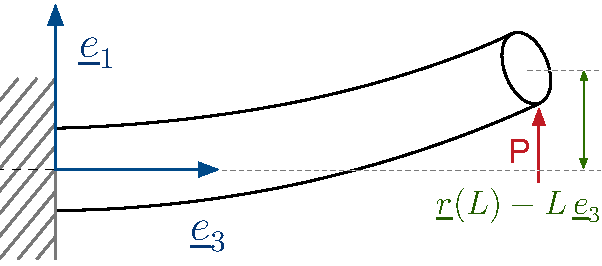
\includegraphics[width=14cm, keepaspectratio=true]{sections/cosserat_rods/images/MinimumPotentialEnergyMethodExample}
  \end{figure}
\end{frame}